\documentclass[tikz,convert={outfile=foldNatFree-mmorph-unit.svg}]{standalone}
\begin{document}
\tikzstyle{every node}=[font=\footnotesize]
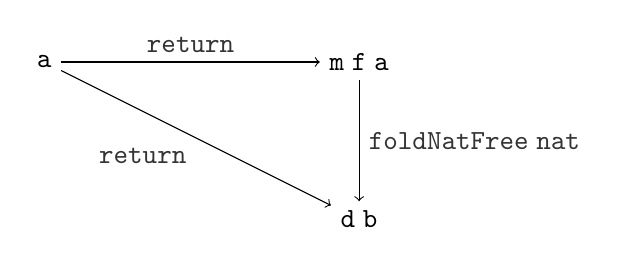
\begin{tikzpicture}
    \node (A) at (0,2) {$\mathtt{a}$};
    \node (B) at (4,2) {$\mathtt{m}\;\mathtt{f}\;\mathtt{a}$};
    \node (D) at (4,0) {$\mathtt{d}\;\mathtt{b}$};
    \draw[->] (A) -- node[above] {\textcolor{black!80}{$\mathtt{return}$}} (B);
    \draw[->] (B) -- node[right] {\textcolor{black!80}{$\mathtt{foldNatFree}\;\texttt{nat}$}} (D);
    \draw[->] (A) -- node [below left] {\textcolor{black!80}{$\mathtt{return}$}} (D);
\end{tikzpicture}
\end{document}
